%\documentclass[a4paper,12pt,draft]{report}% ,draft
\documentclass[a4paper,12pt]{report}
\usepackage[hyphens]{url}
\usepackage{xunicode}
\usepackage{xltxtra}
\usepackage[slovak,english]{babel}
\usepackage{lastpage}
\usepackage{graphicx}
\usepackage{color}
\usepackage[colorlinks]{hyperref}
\usepackage{lmodern}
\hypersetup{linkcolor=black, urlcolor=blue, citecolor=black}


%\usepackage[left=3cm,right=2cm,top=2.5cm,nohead,foot=1.0cm]{geometry}

\usepackage[left=3.5cm,right=2cm,top=2.5cm,nohead,foot=2.5cm]{geometry}

%\usepackage[left=3cm,right=3cm,top=3cm,nohead,foot=3cm]{geometry}

% A4 is 297x210 mm

%\setlength{\textwidth}{160mm}
%\setlength{\textheight}{240mm}
% textheight should be 246, but some printers have problems printing
% at the bottom of the page

\renewcommand{\baselinestretch}{1.5}
%\setcounter{tocdepth}{1} %hlbka obsahu

\author{Dušan Ščensný}
\title{Bakalárska Práca}
%\setcounter{page}{0}


\begin{document}

%Úvodná časť záverečnej práce obsahuje tieto položky v danom poradí:
%(7)   obal,
%(8)   titulný list,
%(9)   zadanie záverečnej práce,
%(10)                      poďakovanie (nepovinné),
%(11)                      abstrakt v štátnom jazyku,
%(12)                      abstrakt v anglickom jazyku, resp. inom cudzom jazyku,
%(13)                      obsah,
%(15)                      zoznam skratiek a značiek (v technických a prírodovedných odboroch povinné),

\begin{titlepage}
\begin{center}
% Upper part of the page
%\includegraphics[width=0.5\textwidth]{./logo}\\[1cm]

\textsc{\LARGE Žilinská Univerzita v~Žiline\\ Fakulta riadenia a informatiky}\\[3.5cm]%[1.5cm]
% text small caps

\textsc{\Large Bakalárska práca}\\[0.5cm]
{ \large \bfseries Študijný program: informatika}\\[1.5cm]%[0.9cm]
% \bfseries = Boldface. alebo \textbf
\end{center}

\vfill
% urobi co najviac volneho miesta vertikalne
\begin{center}
\textbf{Dušan Ščensný}\\
%\large vedúci: Mgr. Michal \textsc{Kaukič}, CSc.\\
%\large číslo : \\
\end{center}
%\begin{flushleft}
\begin{center}
%\hspace{3.0 cm} 
\textbf{Softvér pre komunikáciu s GPS modulom} \\
\textbf{a zobrazovanie GPS dát}\\
\end{center}
\begin{center}
\textbf{Vedúci: Mgr. Michal \textsc{Kaukič}, CSc.}\\ 
Reg.č. 77/2009 \hspace{3.0cm}    Máj 2010\\
\hspace{2cm}\\
\end{center}
\end{titlepage}

%\beg
\chapter*{PREHLÁSENIE}
\thispagestyle{empty}
%\vfill
\vspace{12cm}
Prehlasujem, že som bakalársku prácu spracoval samostatne a že som uviedol všetky použité pramene a literatúru, z ktorých som čerpal.

\vspace{2cm}
\noindent
V Žiline dňa \makebox[8em]{\dotfill} \hfill Podpis\makebox[8em]{\dotfill}

%\chapter*{Poďakovanie}
%\thispagestyle{empty}


%vytvorenie titulky , so zarovnanim
%\title{The Triangulation of Titling Data in       Non-Linear Gaussian Fashion via $\rho$ Series}
%\date{October 31, 475}
%\author{John Doe\\ Magic Department, Richard Miles University
 %       \and Richard Row, \LaTeX\ Academy}

%Abstrakt obsahuje informáciu o cieľoch práce, jej stručnom obsahu a v závere abstraktu sa charakterizuje splnenie cieľa, výsledky a význam celej práce. Súčasťou abstraktu je 3 - 5 kľúčových slov. 
\selectlanguage{slovak}
\begin{abstract}
\textsc{Ščensný}, Dušan: \emph{Softvér pre komunikáciu s GPS modulom a zobrazovanie GPS dát}[bakalárska práca] - Žilinská Univerzita v~Žiline. Fakulta riadenia a informatiky; Katedra matematických metód. -Vedúci: Mgr. Michal Kaukič, CSc. - Stupeň odbornej kvalifikácie:Bakalár v~odbore Informatika. Žilina: FRI ŽU v~Žiline, 2010. - \pageref{LastPage} s.
\\*[1.0cm]
Cieľom tejto bakalárskej práce bolo vytvoriť robustnú aplikáciu, ktorá má komunikovať s GPS prístrojom a zobrazovať GPS dáta. Obvykle sú dáta vo forme trás a významných bodov, ktoré musia byť ukladané v pamäti konkrétnou údajovou štruktúrou.  Základné funkcie GPS systému a práca s geografickými dátami sú podrobne vysvetlené, pretože sú dôležité pre pochopenie systému navigácie a prepočtov potrebných pri vykresľovaní dát. Vo výslednej aplikácii bola použitá knižnica Qt pomocou ktorej bolo vytvorené jadro aplikácie aj grafické rozhranie. Vývoj tejto aplikácie podnietilo hlavne to, že na trhu je nedostatok takýchto produktov ktoré sú jednoduché, rýchle a bezplatné. Aplikácia sa dá považovať za prvú fázu vo vývoji v ktorej sú implementované základné prvky softvéru pracujúceho s GPS prístrojom a samotnými mapami.\\[1.0cm]
\textbf{Kľúčové slová:} GPS, Qt, Aplikácia, prístroj
\end{abstract}

\selectlanguage{english}
\begin{abstract} 
%\textbf{Abstract}\\
%\end{center}
\textsc{Ščensný}, Dušan: \emph{Software for communication with GPS module and GPS data visualization.}[Bachelor thesis] - University of Žilina. Faculty of Management Science and Informatics;Department of mathematical methods - Tutor: Mgr. Michal Kaukič, CSc. - Qualification level:Bachelor in field Informatics. Žilina: FRI ŽU v~Žiline, 2009. - \pageref{LastPage}~p.
\\*[1.0cm]
The object of this Bachelor thesis was to create a robus application, which comunicates with GPS device and displays the GPS data. Ususally are data in form of tracks and waypoints, which must be saved in memory in concrete data structure. The basic functions of GPS system and work with geographical data are in details explained, because of their important for comprehension of system navigation and calculation needed by drawing data. In final application were used library called Qt by which were created core of application and a graphical interface. Development of this application in main motivate, that at market is lack of this products which are simple, fast and free. Application can be consider in first phase at our development in which are implemented the basic component of software work with GPS device and maps.\\[1.0cm]
\textbf{Keywords:} GPS, Qt, application, device
\end{abstract}

\selectlanguage{slovak}
%Predhovor je povinný vo všetkých kvalifikačných prácach. Píše sa spravidla na jednej samostatnej strane. Autor uvedie hlavné charakteristiky práce. Stručne informuje, čo je hlavná téma a aké dôvody viedli autora k voľbe témy. Načrtne domáci a zahraničný kontext,informuje ako a kým by sa práca mohla použiť. Informuje tiež o tom, kto autorovi poskytol pomoc a ak to uzná za vhodné, poďakuje im.

\section*{PREDHOVOR}
\paragraph{}
Práca s mapami fascinovala už mnoho ľudí. Dôvod pre spracovanie tejto témy bol dlhodobý záujem o prácu s mapami a mapovým softvérom, tiež záujem o hlbšie poznanie GPS princípov a častí ktoré vo všeobecnosti nie sú známe. 

V úvode tejto práce nájdeme stručne popísaný prechod z histórie až po súčasnosť a zároveň stručný popis výberu softvéru, ktorý je dôležitý pri vývoji a tiež softvéru ktorý je vhodný použiť pri práci s dátami. 

V prvých troch kapitolách sú popísané základné prvky týkajúce sa geografie, kartografie a s ňou spojenej projekcie zemského povrchu do mapy. Následne sa v týchto kapitolách pojednáva o fungovaní GPS\footnote{\textbf{GPS} - globálny pozičný systém}, ktorý je dôležitou súčasťou tejto práce. S navigačnými prístrojmi sa blízko spája protokol NMEA\footnote{\textbf{NMEA} - národná vojenská asociácia pre elektroniku (national marine electronic association)} ktorý sa často používa ako základ pri prenose údajov z prístroja do počítača alebo priamo do softvéru. Programy ktoré sa používajú pri konvertovaní dát často používajú ako prenosový formát GPX\footnote{\textbf{GPX} - GPS eXchange format = formát na výmenu dát}. S formátom sa oboznámime v druhej kapitole. V práci nájdeme aj popis prístrojov na ktorých bola testovaná komunikácia softvéru. 

Posledná kapitola sa zaoberá vytvoreným softvérom OSM\_Navigation, popisom jeho hlavných častí, ako aj vysvetlenia konkrétnych prvkov použitých pri práci. V tejto kapitole sa nachádza postup na kompiláciu programu, vytváranie závislostí ako aj popis jednotlivých tried nachádzajúcich sa v programe. Softvér je použiteľný pre široké spektrum používateľov a to aj z toho dôvodu že nie je zameraný na konkrétny typ prístrojov.

\paragraph{}
Rád by som poďakoval všetkým, ktorí mi pri tvorbe bakalárskej práce pomohli, či 
už cennými radami, pripomienkami, zapožičaním prístrojov alebo pomocou pri zhromažďovaní materiálov. 
Predovšetkým však poďakovanie patrí vedúcemu bakalárskej práce \mbox{Mgr.~Michalovi Kaukičovi,~CSc.}
	% titulna strana, abstrakt, podakovanie
\thispagestyle{empty}
\renewcommand\thepage{}
\tableofcontents	% obsah 
\newpage
\renewcommand\thepage{\arabic{page}}
\chapter*{ÚVOD}
\addcontentsline{toc}{chapter}{Úvod}
%V úvode autor stručne a výstižne charakterizuje stav poznania alebo praxe v oblasti, ktorá je predmetom záverečnej práce a oboznamuje čitateľa s významom, cieľmi a zámermi práce. Autor v úvode zdôrazňuje, prečo je práca dôležitá a prečo sa rozhodol spracovať danú tému. 
%\section{GPS prístroje}
\paragraph{} 
Prácou s mapami sa zaoberali ľudia už v staroveku, z dôvodu zachytenia prvkov nachádzajúcich sa v okolí. Jeden z dôvodov bol, že mapa nás priviedla vždy do cieľa, na miesto kde sme sa chceli dopraviť. Mapy sa využívali a využívajú všade okolo, môžeme to vidieť v histórii ale aj v aktuálnej dobe.

V súčasnosti je snaha zachytiť každučký detail na mape, vecí a okolnosti ktoré nás zaujímajú, ktoré sú pre nás podstatné. K tomu aby sme mohli zaznamenať na mape rôzne detaily, nás rapídne posúva vpred elektronika z takzvaným GPS systémom. Za posledné dva desaťročia sa trh s touto elektronikou rapídne rozšíril, no nebolo tomu vždy tak. 

GPS je skratka pre Globálny pozičný systém, ktorý vyvinula Americká vláda počas studenej vojny. V časoch studenej vojny mal tento systém úplne iný zmysel ako dnes, jeho vývoj napredoval hlavne ako konkurencia Ruskej vláde a jej vývoju. Časté názory na vývoj GPS sú práve tie že s týmto systémom začala USA a je to aj pravda, ale prvý rádiofrekvenčný signál ktorý tento vývoj podnietil prišiel práve z ruskej družice a tak istý podiel na tomto systéme má určite aj Rusko. Americká vláda s vývojom systému napredovala vred. Dnes je tento navigačný systém jediný na trhu dostupný pre verejnosť, ale je všeobecne známe že funkčných pozičných systémov je omnoho viac, ktoré ale pre verejnosť dostupné nie sú. 

Tento navigačný systém je spustený od roku 1960 a od vtedy prešiel dlhým vývojom, až po dnešnú podobu. Verejnosti bol sprístupňovaný od roku 1990 do roku 1993 po tomto roku už bol plne prístupný. Americká vláda mala obavy o zneužitie systému a tak až do roku 2000 bola v navigačnom systéme zavedená funkcia selektívnej dostupnosti\footnote{\textbf{selektívna dostupnosť} - "Zámerné znepresnenie polohy pre civilných užívateľov GPS, selektívna dostupnosť ang. Selective Availability (SA)" [10]}, ktorá degenerovala presnosť na +-200 metrov. Po zrušení funkcie je dnešná presnosť týchto hodnôt na niekoľko metrov a v špeciálnych geodetických prístrojoch dokonca niekoľko centimetrov. 

Vzhľadom na dostupnosť signálu sa prudko rozšíril aj trh s príjmačmi, následkom čoho bol dopyt po softvéroch ktoré by boli schopné tieto dáta zobrazovať. Bežnou požiadavkou používateľov bolo aby bol systém schopný ukladať body alebo trasy, aby ich bolo možné neskôr nájsť. Na to aby sme to dokázali nám vystačí aj lacnejší a tým aj dostupnejší prístroj pre širokú verejnosť, ktorá ho môže využiť na navigovanie, alebo ukladanie dát.

Podnet na výber tejto témy bol hlavne z tohto dôvodu: Prístrojov na navigáciu je široké spektrum, ale naozaj kvalitný softvér pre široké spektrum užívateľov chýba. Cieľ tejto práce ale nebol vyvinúť softvér so všetkými funkciami o ktoré používateľ má záujem, pretože by nato nebol dostatok času počas jednej práce. Snahou bolo vytvoriť základ pre ďalší, kompletnejší vývoj softvéru.
Ďalším dôvodom pre spracovanie danej témy bolo vytvoriť si rozhľad medzi už dostupným softvérom\footnote{\textbf{softvér} - je označenie pre programové vybavenie počítača} a hardvérom\footnote{\textbf{hardvér} - tu patria všetky počítače a ich súčasti, periférie (zobrazovacie jednotky, zariadenia na vstup a výstup údajov)} GPS.

\section*{Výber softvéru}
\paragraph{}
Pri výbere softvéru sa často stretávame s problémom nekompatibility s
operačným systémom. Dnes máme dostupné rôzne navigačné aplikácie pod OS\footnote{\textbf{OS} - Operačný systém} Windows
ktoré ale nie je možné používať pod OS Linux, alebo inými. Tento problém nám môže vyriešiť
správna voľba programovacieho jazyka a vývojového prostredia. 
V tejto práci sme sa zameriavali na OS Linux, no pri výbere programovacieho
jazyka, ako aj vývojového prostredia sme kládli dôraz na kompatibilitu s inými
OS aby pri budúcom pokračovaní na tomto projekte ho bolo možné zdieľať aplikáciu širokou verejnosťou. 
	% Úvod
\chapter{Geografické údaje}
\section{\textsc{Základné pojmy v geografii}}
\paragraph{}
V tejto podkapitole sa vysvetľujú pojmy týkajúce sa geografie, súvisiacej z GPS prístrojmi a súradnicami.
\paragraph{Súradnicový systém}
" je vzájomne jednoznačné zobrazenie medzi množinou bodov n-rozmerného priestoru
a usporiadanou n-ticou skalárov (veličín či čísiel; spravidla reálnych čísiel).
Tieto skaláre (pri ktorých záleží na poradí v ktorom sú uvádzané) sa nazývajú
súradnice alebo koordináty."[2]%" [Marián Jurík]
\paragraph{WGS-84}
\footnote{\textbf{WGS-84} - World Geodetic System 1984}
"WGS 84 je pravotočivá karteziánska sústava súradníc so stredom v ťažisku Zeme (vrátane morí a atmosféry). Kladná os x smeruje ku priesečníku nultého poludníka a rovníka, kladná os z ku severnému pólu a kladná os y je na obe predchádzajúce kolmá v smere doľava (90° východnej dĺžky a 0° šírky), tvorí tak pravotočivú sústavu súradníc"[12]

\begin{figure}[ht]
\centering
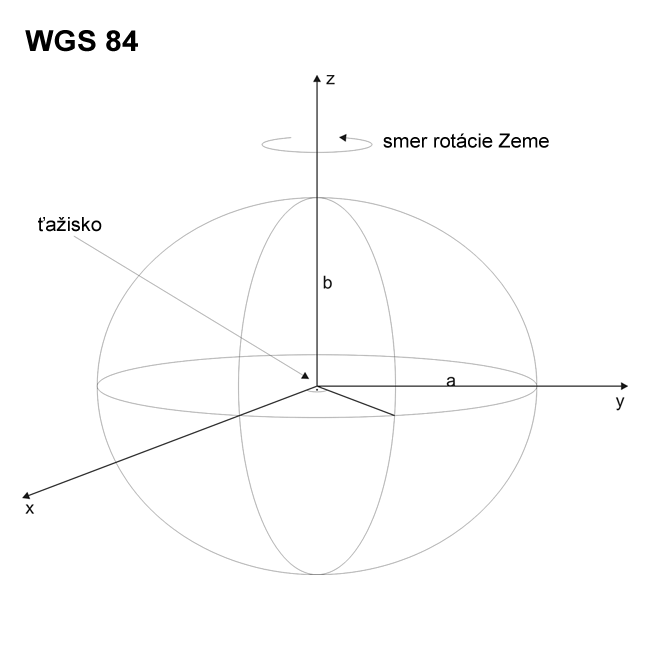
\includegraphics[height=9.0cm]{obr/Wgs84}
\caption{Systém udávania súradníc}
\end{figure}

\paragraph{}\paragraph{}\paragraph{}%\paragraph{}
\section{\textsc{Kartografická projekcia - Zobrazenie Máp}}
\paragraph{}
Prvoradý predpoklad analýzy a tvorby mapových výstupov z geografických
(vektorových\footnote{\textbf{Vektor} - prvok vektorového priestoru (na rozdiel od skaláru je okrem svojej absolútnej hodnoty určený aj smerom a orientáciou)} alebo rastrových\footnote{\textbf{rastrová grafika} - označuje spôsob uloženia grafickej informácie jednotlivých bodov usporiadaných v pomyslenej mriežke}) údajov je, že sa tieto údaje vzťahujú k jednotnému
súradni\-co\-vé\-mu systému (vysvetlený v predošlej kapitole).

Vo väčšine prípadov sú údaje z rôznych mapových podkladov, ktoré boli vyhotovené
v rôznych kartografických zobrazeniach a v rôznych mierkach. Nevyhnutnou
súčasťou procesu tvorby priestorovej databázy a mapových výstupov je preto
transformácia súradníc objektov medzi rôznymi súradnicovými systémami.
Pri spracovaní údajov berieme do úvahy min tri zobrazenia:
zobrazenie vstupných máp, interné zobrazenie (v programe), zobrazenie výstupov (dáta).
Ideálne je keď sa tieto zobrazenia zhodujú čo sa ale nestáva často.

\paragraph{}
\begin{figure}[ht]
\centering
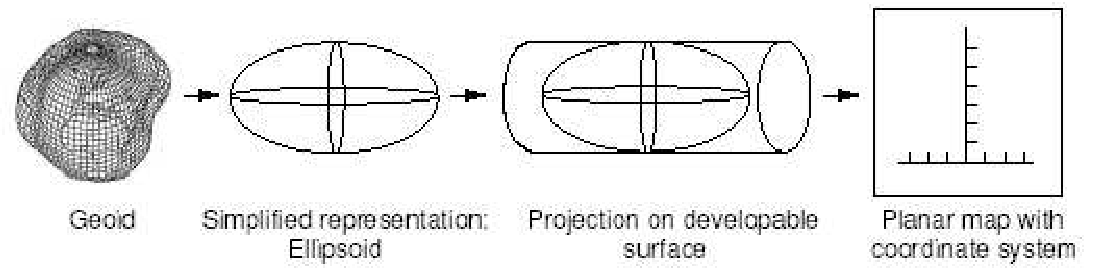
\includegraphics[width=14.5cm]{obr/zem_do_mapy}
\caption{Zpracovanie zemského povrchu do mapového zobrazenia}
\end{figure}

Význam interného kartografického zobrazenia, jednotného súradnicového systému a~presnosti kartografických transformácii rastie priamo úmerne s veľkosťou
spracová\-va\-né\-ho územia a s počtom užívateľov geografickej databázy. Pre
lokálne
databázy prístupne obmedzenému počtu užívateľov (napr. mapa zelene v intraviláne
jednej obce), postačuje zadefinovať lokálny pravouhlý súradnicový systém. Na
malých vzdialenostiach sa zakrivenie zemského povrchu môže zanedbať. Na
zjednotenie máp zelene všetkých obci okresu určite budeme potrebovať
transformáciu do jednotného su\-rad\-ni\-co\-vé\-ho systému. V prípade
medzinárodných
projektov, keď záujmové územie presahuje hranice jedného štátu a databázu
používajú organizácie z rôznych štátov s rôznymi národnými zobrazeniami a
tradíciami, sa vhodné riešenie hľadá ťažko.

\subsection{Referenčný elipsoid} 
Matematická aproximácia tvaru Zeme a iných telies vo vesmíre je referenčným elipsoidom. Skutočný tvar zeme je nepravidelný, no nejedná sa len o hory, kopce ale aj samotné moria sú nepravidelne vzdialené od stredu zeme (geoid viď. obrázok 1.3). Vplýva na to nepravidelné rozloženie hmoty zeme a tým aj rôznymi gravitačnými potenciálmi na zemi. Kľudová vzdialenosť hladiny mora sa môže líšiť na niektorých miestach zeme až o 100 metrov.

Základným súradnicovým systémom na referenčnom elipsoide sú \textbf{zemepisné
sú\-rad\-ni\-ce},
niekedy tiež nazývané geodetické zemepisné, alebo geografické sú\-rad\-ni\-ce.
Sú tvorené \textbf{zemepisnou (geografickou) šírkou a zemepisnou (geografickou) dĺžkou}. Zemepisné poludníky a
rovnobežky vytvárajú na referenčnom elipsoide zemepisnú sieť. Referenčný
elipsoid sa používa pri definícii štátnych a medzinárodných geodetických
súradnicových systémov, pri tvorbe mapových dielov veľkých a stredných mierok,
keď sa vyžaduje minimálne skreslenie.

\begin{figure}[ht]
\centering
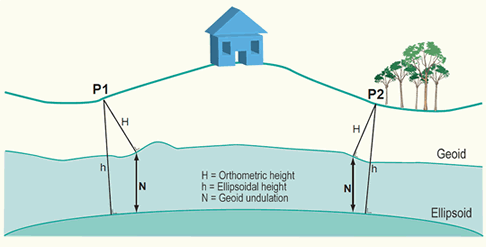
\includegraphics[width=14.5cm]{obr/relationshipse}
\caption{Referenčný elipsoid}
\end{figure}

\section{\textsc{GPS}}
\paragraph{}
"Global Positioning System, zvyčajne nazývaný GPS (armáda USA ho označuje ako
NAVSTAR GPS\footnote{\textbf{NAVSTAR GPS} - NAVigation Signal for Timing And Ranging}), je satelitný navigačný
systém používaný na zistenie presnej pozície a poskytujúci veľmi presnú časovú
referenciu takmer kdekoľvek na Zemi alebo na zemskom orbite. Používa zostavu
aspoň
24 satelitov na strednom zemskom orbite."[11].

Tento navigačný systém je funkčný 24 hodín denne, celý čas dokáže poskytovať údaje. Jedná sa o pasívny dĺžkomerný družicový systém. Cieľom tohto systému je poskytovať údaje o polohe na ktorej sa prijímateľ signálu nachádza. Pôvodne bol určený na vojenské účely, na zisťovanie polohy, rýchlosti a času. Neskôr ale americká vláda rozhodla o sprístupnení GPS signálu pre verejnosť. Systém je dostupný neustále vďaka tomu že jeho družice sú rozmiestnené tak aby v každom okamihu na celej zemi boli dostupné aspoň štyri satelitné prijímače. Štyri práve preto lebo tento signál sa vypočítava zo štyroch veličín (viď obr. 1.1) tieto veličiny sú hodnoty \textit{x,y,z} a posledná potrebná veličina je čas \textit{t}. V špeciálnych prípadoch nám postačujú aj tri veličiny a to vtedy keď máme jednu z veličín známu. Preto známu, lebo niektoré prístroje sú schopné zistiť nadmorskú výšku(pr. systémy na morských lodiach).

\paragraph{Konkurencia}
\begin{enumerate}
\item GLONASS\footnote{\textbf{GLONASS} - Globálny satelitný navigačný systém} - ruský družicový navigačný systém
\item Galileo - výstavbu realizuje Európska únia. Systém Galileo by mal byť prevádzkyschopný od roku 2010.
\item Compass - vyvíjaný Čínou, regionálne používaný pod názvom Beidou
\item DORIS - systém vyvíjaný Francúzskom
\end{enumerate}

\subsection{\textsc{Funkčnosť GPS systému}}
\paragraph{}
"To, čo sa deje v každom GPS prijímači by sme mohli opísať ako určovanie polohy
meraného bodu z priesečníku guľových plôch, ktorých polomer je daný meranými
vzdialenosťami. Tento systém sa nazýva tiež dĺžkomerný systém. Meranou veličinou
je doba šírenia rádiového signálu z družicovej antény k anténe GPS prijímača. Rýchlosť šírenia signálu je rovná rýchlosti svetla. Každá družica v
navigačnej správe okrem iných údajov posiela aj parametre svojej dráhy
z ktorých vieme vypočítať aktuálnu polohu družice (\textit{XS, YS, ZS}). Keď
poznáme súradnice družíc, môžeme polohu užívateľa (\textit{X, Y, Z}) určiť vypočítaním
sústavy troch rovníc o troch neznámych. Problém merania polohy by bol
jednoduchý, keby časové základne (hodiny) družice a užívateľa boli synchrónne.
Hlavný problémom je doba, ktorá uplynie medzi vyslaním diaľkomerného signálu z
GPS družice a jeho prijatím užívateľským GPS prijímačom. Časová základňa
užívateľského zariadenia je posunutá o neznámy časový interval \textit{Dt}, ktorý môžeme
prepočítať na vzdialenosť \textit{b = c Dt} (kde c je rýchlosť svetla). K neznámym
súradniciam užívateľa pristupuje teda neznáma \textit{b} a pre výpočet polohy potrebujeme
celkom štyri rovnice

\begin{verbatim}
(xi - x)2 + (yi - y)2 + (zi - z)2 = Di + b
Di = c tmi
i = 1, 2, 3, 4   "[11].
\end{verbatim}

\section{\textsc{Možnosti zobrazenia máp}}
\subsection{On-line mapy} 
\paragraph{}
Vo všeobecnosti majú veľké množstvo dát. Tieto mapy sú rozdelené na
množstvo fotografií ktoré sú kalibrované GPS súradnicami tak aby tvorili jeden
celok. Počet obrázkov na ktoré sú rozdelené je určený priblížením. Každý obrázok
má konštantnú veľkosť v pixloch. Mapy ktoré vidíme sú delené, na konštantnú
veľkosť. Čím je priblíženie väčšie tým je počet obrázkov väčší. Pri
pohľade na mapu vidíme, že približovaním sa zväčšuje detail na mape. Väčšina
užívateľov si pritom vôbec neuvedomí že priblížením sa pozerá na úplne inú
fotografiu = mapu rovnakú no z väčším počtom detailov. 
\paragraph{}
V súčasnosti máme možnosť výberu rôznych dostupných on-line máp. Medzi najznámejšie partia:
\begin{list}{•}
\item OpenStreetMap
\item
\item GoogleMaps
\item MapQuest
\item Yahoo! Maps
\item Multimap.com (Spojené kráľovstvo)
\item Map24
\end{list}

Každé majú svoje výhody aj nevýhody. V nasledujúcej podkapitole budú niektoré popísané.

\subsection{\textsc{Spôsob sťahovania konkrétnych častí mapy}}
\paragraph{}
Keďže mapu nemáme dostupnú celú, musíme pri pohybe priebežne sťahovať jednotlivé jej časti. Avšak je nutné vykonať istý numerický prepočet. Tento prepočet sa vykoná podľa
aktuálnej pozície GPS. Pri prepočte musíme zohľadniť priblíženie, veľkosť
obrázka a samotné súradnice.\\\\
Pri sťahovaní obrázka zo serveru zadávame do adresy tri hodnoty:
\begin{list}{•}
\item prepočítanú zemepisnú šírku
\item
\item prepočítanú zemepisnú dĺžku 
\item hodnotu priblíženia (zvyčajne hodnoty 2-17)
\end{list}

Dostupnosť maximálneho priblíženia určuje typ on-line mapy, rôzne on-line mapy
môžu mať rôzne priblíženie.

\subsection{\textsc{Google Mapy}}
\paragraph{Google maps}
 "je bezplatná, on-line mapová služba spoločnosti Google. Ponúka
posú\-va\-teľ\-né mapy a satelitné snímky celého sveta...

Označenie „satelitné snímky“ však nie je celkom presné, pretože časť záberov s
najväčším rozlíšením (prevažne z územia USA, ale aj napr. z Paríža) pochádza z
leteckého snímkovania."[5]

\subsubsection{Satelitná snímka} 
Tento pojem je vlastne fotografia fotená (snímaná) zo satelitu z výšky približne niekoľko tisíc metrov. Táto fotografia je následne spracovaná kalibráciou\footnote{\textbf{Kalibrácia} - je určenie presných súradníc kalibračných bodov} následne je možné mapu použiť na navigáciu príp. určenie polohy. Takýmito mapami disponuje aj spoločnosť Google, pod názvom "GoogleMaps".\\\\\\

Satelitné snímky existujú v dvoch typoch:
\begin{enumerate}
\item Snímky s komerčného satelitu QuickBird, ktoré sú schopné snímať plochu o rozmeroch (16,5 x
16,5) km. Maximálne rozlíšenie týchto snímok je 60 cm na pixel\footnote{\textbf{pixel} - skratka z angl. picture element - obrazový prvok} (viď. obrázok 1.4). Počas jedného snímania je satelit schopný spojiť až 10 snímok čím vznikne výsledný snímok o veľkosti (16,5 x 165) km 

\item Snímky z Amerického programu Landsat, ktorý pracuje od roku 1972. Najnovší satelit, ktorý pracuje v rámci tohto programu je Landsat 7. Tento satelit je schopný snímať maximálnu plochu o rozmeroch (185 x 185) km. Pracuje s rozlíšením 15 m na pixel. Zem je takto neustále snímaná až do súčasnosti.
\end{enumerate}

\begin{figure}[ht]
\centering
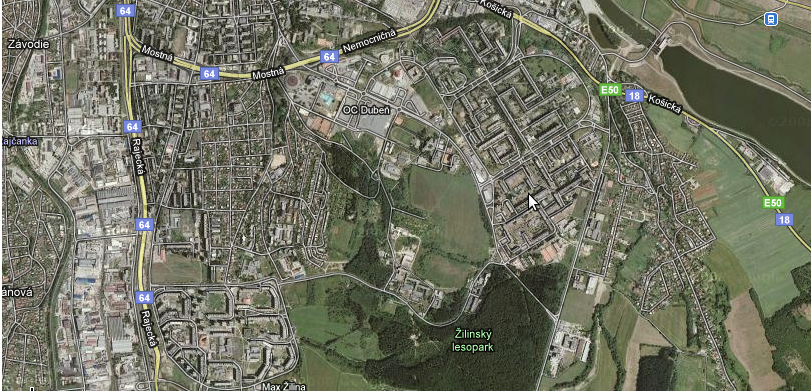
\includegraphics[width=14.5cm]{obr/gogmaps}
\caption{Príklad zobrazenia Google Máp}
\end{figure}

\subsection{\textsc{OpenStreetMap}}
\paragraph{OpenStreetMap(OSM)}
  "je otvorený projekt, ktorého cieľom je tvorba voľných
geografických dát, ako sú napríklad cestné mapy. Používa predovšetkým dáta z
prijímačov GPS (v režime automatického zaznamenávania súradníc prechádzanej
trasy), ktoré sú následne kontrolované a editované. Je založený na kolektívnej
spolupráci a na koncepcii Open source\footnote{\textbf{Open source} - voľne šíriteľný}."[9].

Tvorba máp a zaznamenávanie ciest do máp sa dá považovať za úspešné vzhľadom na to, že počet používateľov týchto máp stále stúpa. Značne množstvo ľudí láka hlavne to že do tvorby máp sa môžu zapojiť a tak si môžu vytvárať mapy svojho okolia, ktoré následne môže využiť ktokoľvek. OpenStreetMap je nezisková organizácia, ktorej zakladateľ je Steve Coast. Ako organizácia sa tento projekt označuje od roku 2006. Všetky tieto dáta je možné upravovať používateľmi máp. Nato aby sme mohli dáta do databázy nahrávať a aby sa mohli neskôr porovnať je potrebné sa zaregistrovať na stránke \url{http://www.OpenStreetMap.org}. \\
Slovenská stránka pre OSM je \url{http://www.freemap.sk/}


\paragraph{Šírka záberu} Mapovacie rozhranie zhŕňa síce celý svet ale hlavné body pre mapovanie sa odohrávajú vo Francúzku, Škandinávii, na ostrove Man a v Spojenom kráľovstve. Dáta z územia USA pochádzajú z databázy TIGER\footnote{\textbf{TIGER} - vytvorené pri sčítaní ľudu}. 

\begin{figure}[ht]
\centering
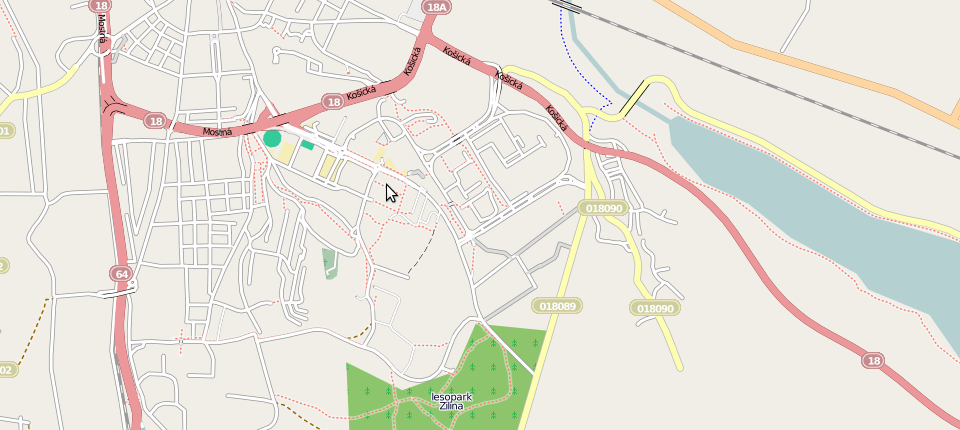
\includegraphics[width=14.5cm]{obr/osm}
\caption{Príklad zobrazenia Open Street Map}
\end{figure}

\paragraph{Zdroj dát} nie sú ako by sme možno očakávali z konkrétnej firmy alebo organizácie, ale od bežných používateľov ktorý si svojvoľne snímajú dané trasy. Tieto trasy následne prejdú analýzou a po zhodnotení (porovnaní so satelitnými snímkami družice Landsat7) sa dané trasy zapíšu do mapy. Týmto spôsobom je zaistený ich skutočný stav ich umiestnia.
   	% Možnosti zobrazenia máp
%podkapitoly
%\section{Protokol NMEA 0183}
%\section{Formát GPX}
%\section{GPS babel}
%\section{Gps multi tracker}

\chapter{Spracovanie dát z GPS prístroja}

\section{Protokol NMEA 0183}
\paragraph{NMEA}
"Štandardizovaný komunikačný protokol pre prenos dát z GPS do iného
elektronického zariadenia (najčastejšie PC) v reálnom čase. Dáta z GPS sú
tematický rozdelené do niekoľkých skupín - ASCII reťazcov a posielané von
z prístroja."[10]

Tento protokol na najčastejšie používa pre prenos GPS dát potrebných na zobrazenie pozície používateľa, ktorý smeruje z prístrojov do PC zariadení.
Každá veta začína znakom \$. Za znakom \$ pokračuje označenie dát, za ktorým sa nachádzajú konkrétne dáta. Dáta sú oddelené čiarkou, pre dobré rozonanie. V prípade že sa konkrétne dáta nedajú vypočítať (nedostupnosť signálu, nedostatok dát potrebných pre výpočet) sú prístrojom na danej pozícii posielané ako nuly ako prázdne dáta.  Niektoré prijímače neposielajú všetky dáta.

\paragraph{Popis NMEA prvkov}
Pred každý z kódov sa pridáva príznak GP\\
RMB  = Minimálne potrebné navigačné informácie\\
RMC  = Odporúčané minimálne tranzitné údaje \\
GGA  = Globálny pozičný systém Fixné dáta(zemepisné súradnice, nadmorská výška, počet satelitov a pod.)\\
VTG  = Kvalita a rýchlosť aktuálnej trate\\
RMA  = Minimálne potrebné navigačné informácie\\
%GSA  = mód GPS prijímača, SVs a DOP hodnoty\\
GSV  =  Viditeľné Satelity\\
\begin{center}
 \textbf{Príklad NMEA dát}
\begin{verbatim}
Dáta sú dostupné:
$GPGGA,110532.538,4910.1966,N,01852.6027,E,0,00,1.4,2.5,M,44.0,M,,00*57
$GPVTG,161.5,T,,M,043.8,N,081.1,K,N*06

Dáta nie sú dostupné:
$GPGGA,185837.507,0000.0000,N,00000.0000,E,0,00,50.0,0.0,M,0.0,M,,00*74
$GPRMC,185837.507,V,0000.0000,N,00000.0000,E,,,050309,,*19
\end{verbatim}
\end{center}

\section{Formát GPX}
\paragraph{}
Bol navrhnutý tak, že dáta sú uložené v XML formáte. Tento formát má veľa
výhod. GPX (z angl. GPS eXchange Format) je formát súborov pre ukladanie dát vo forme HTML tagov\footnote{\textbf{tag} - značka metadát}. Dáta sú tak vhodné do spracovania počítačom, ale zároveň sú jednoducho čitateľné aj pre človeka. Tento formát je určený hlavne na komunikáciu internetových webov. 

Forma GPX vychádza z XML\footnote{\textbf{XML} - rozšíriteľný značkovací jazyk (eXtensible Markup Language)} formátu. Tento formát sa vyvinul z hlavne html štandardu. Vznikol hlavne preto, lebo samotný html formát postupom času nabral na zložitosti a množstve príkazov. XML formát nemá predpísané značky (tagy), no zároveň jeho syntax je podstatne prísnejšia ako u HTML\footnote{\textbf{HTML} - Hypertextový značkový jazyk HyperText Markup Language)} dát.
\paragraph{}
\textbf{Existujú dve verzie tohto formátu a to:}
\begin{list}{•}
\item 1.0 používaná od roku 2002
\item
\item 1.1 používaná od 9. Augusta 2004 
\end{list}
\paragraph{}
\textbf{Verzie sú vzájomne kompatibilné. Verzia 1.1 priniesla nasledujúce zmeny:}
\begin{list}{•}
\item tagy s obecnými informáciami o celom súbore sa presunuli do tagu metadata
\item
\item miesto tagov url a urlname sa používa nový tag link
\item voliteľné rozširujúce tagy sa presunuli do tagu extension
\end{list}

Programy by mali jasne deklarovať s ktorou verziou GPX vedia pracovať, aby sa
predišlo situáciám kedy nebude možné niektoré GPX dáta spracovať kvôli
nekompatibilite verzie.

\subsection{Element gpx}

\begin{center}
\textbf{Tento element je koreňovým elementom GPX dokumentu}
\begin{verbatim}                                                    
"< gpx
   version = " 1.1 [1] "
   creator = " xsd:string [1] " >
       < metadata > metadataType </ metadata > [0..1]
       < wpt > wptType </ wpt > [0..*]
       < rte > rteType </ rte > [0..*]
       < trk > trkType </ trk > [0..*]
       < extensions > extensionsType </ extensions > [0..1]
</ gpx > "[2]
\end{verbatim}
\end{center}
Hodnoty v zátvorkách znázorňujú početnosť dát v zázname. Každý začiatočný tag musí mať aj svoju ukončovaciu značku.\\


\begin{center}
\textbf{Príklad GPX schémy typu waypoint}
\begin{verbatim}
<wpt lat="49.210526565" lon="18.758500053">
  <ele>435.097072</ele>
  <time>2009-10-29T21:50:20Z</time>
  <name>TP1149</name>
  <cmt>TP1149</cmt>
  <desc>TP1149</desc>
</wpt>
\end{verbatim}
\end{center}

Jednotlivé tagy môžu obsahovať niektoré z atribútov(pr: `lat`,`lon`). Samotné atribúty majú len názvy (žiadne začiatočné ani ukončovacie značky). Názvy tagov sú vždy na začiatku a na konci(pr: `ele`,`wpt`). Tagy musia obsahovať aj začiatočné aj ukončovacie značky.


\begin{center}
\textbf{Príklad GPX schémy typu track}
\begin{verbatim}
<...>
<name> xsd:string </name> [0..1] ?
<cmt> xsd:string </cmt> [0..1] ?
<desc> xsd:string </desc> [0..1] ?
<src> xsd:string </src> [0..1] ?
<link> linkType </link> [0..*] ?
<number> xsd:nonNegativeInteger </number> [0..1] ?
<type> xsd:string </type> [0..1] ?
<extensions> extensionsType </extensions> [0..1] ?
<trkseg> trksegType </trkseg> [0..*] ?
</...>
\end{verbatim}
\end{center}

V príklade sú dáta iba popisom(informáciou o trase. Popisy nám slúžia na identifikáciu trasy, pričom existencia jednotlivých  popisov je podmienená typom prístroja, ktorý dáta zapisuje. Samotné dáta trás potrebné na vykreslenie sa nachádzajú v časti \textit{trkseg} (názov trksegType v príklade).

\section{Skytraq datalogger}
\paragraph{}Program vyvíjaný Jesper Zedlitz-om, je schopný spracovať dáta z
prístroja s identickým názvom. Tieto dáta ukladá do výstupného formátu GPX.
Samotný vývoj softvéru prešiel pod program GPSbabel, no doposiaľ je iba v testovacej verzii. Tento program nemá GUI interface a spúšťanie prebieha iba v termináli. S programom je možné konfigurovať daný prístroj čo je dôležité pri zapisovaní(logovaní) trás do prístroja. Viac informácii o konfigurácii prístroja sa nachádza v tretej kapitole.
\begin{center}
 \textbf{Vzorové príkazy:}
\begin{verbatim}
skytraq-datalogger --info
skytraq-datalogger <OPTIONS> ACTION
skytraq-datalogger --dump > vystup.gpx 
- uloží výsledné dáta do súboru vystup.gpx
\end{verbatim}
\end{center}
\paragraph{}Všetky ostané informácie sa vypíšu po príkaze info. Používateľ si intuitívne dokáže zvoliť nastavenia prístroja.
Časť options je nepovinná(nastavenia prístroja), no v nasledujúcej časti zadávame žiadanú akciu(`--info`,`--dump`).

\section{GPS babel}
\paragraph{}GPSbabel konvertuje dáta medzi GPS prijímačmi a mapovými programami. Tiež je
vhodný na manipuláciu s týmito dátami.
Tento program umožňuje prácu s dátami priamo na úrovni hardvéru t.j. prácu
priamo s GPS prijímačmi. Podpora dátových formátov stále stúpa a je dostupný pod
rôznymi operačnými systémami.
Nekonvertuje ani neposiela mapy. Pracuje len s dátami ktoré sú na mape uložené,
dátami ako trasami a zaujímavými bodmi. 
Pre túto prácu ho bolo vhodné použiť práve preto, že je dostupný pod rôznymi platformami\footnote{\textbf{platforma} = operačný systém}.
Komunikácia s prístrojom používaným v tejto práci - Sky\_traq data
logger bola nedávno implementovaná. Predchádzajúci softvér postačoval
na nastavenie komunikácie sťahovanie dát, no nebolo s ním možné nastaviť cieľový
bod potrebný na navigáciu s prís\-tro\-jom.
Aby sme mohli použiť tento program museli sme nainštalovať beta verziu programu,
pretože stabilná verzia doposiaľ, nepodporovala tento prístroj.

\subsection{Príkazy v programe GPSbabel}
\paragraph{}Keďže s programom GPSbabel sa pracuje na úrovni príkazového riadku príkazy na
konfiguráciu sú zadávané takýmto spôsobom:

\begin{center}
\textbf{Príkaz na sťahovanie dát}
\begin{verbatim}
gpsbabel -i skytraq,erase -f /dev/ttyUSB1 -o gpx -F suradnice/ke_1.gpx
\end{verbatim}
Príkazom žiadame zariadenie o dáta ktoré budú zároveň zo zariadenia vymazané.
\paragraph{}
\textbf{Príkaz na nastavenie cieľového bodu}
\begin{verbatim}
gpsbabel -i skytraq,targetlocation=49.56:18.21 -f 
    /dev/ttyUSB 0 -o unicsv -F -  
\end{verbatim}
\textbf{syntax:} gpsbabel = názov programu\\
-i = input - vstupný typ súboru/prístroja\\
-f = file - cesta k súboru\\
-o = output - typ výstupného súboru \\
-F = File názov súboru do ktorého sa dáta zapíšu\\
\end{center}

Je nutné podotknúť že vzorové príkazy boli zamerané na konkrétne prístroje ktoré boli v práci používané.

\subsection{Gebabbel}
Tento program je vytvorený ako nadstavba na program GPSbabel. Hlavnými črtami tohto programu je jednoduchosť a jednoúčelnosť. Je vhodným nástrojom na sťahovanie dát a komunikáciu s prístrojmi. Výhodou tohto programu je výber prístrojov, dát a akcií, ktoré sa majú vykonať. Program disponuje aktuálnou databázou prístrojov a formátov, ktoré GPSbabel podporuje.
   	% Spracovanie dát z GPS prístroja
\chapter{GPS prístroje použité v práci}
\paragraph{}
V GPS prístrojoch nastal široký rozmach práve v dnešných časoch. Máme dostupnú
širokú škálu prijímačov z rôznymi presnosťami a to od 10 metrov až po niekoľko
milimetrov. V prístrojoch je snaha o čo najpresnejšie dáta, ale z čo možno najnižšou spotrebou energie pre zaistenie čo najdlhšieho času snímania dát. V tejto práci sme mali k dispozícii dva prístroje ktoré boli od seba značne
odlišné.

Prvý prístroj mal v sebe zabudovanú vnútornú pamäť a dokázal zapisovať prejdené dáta, zobrazovať aktuálnu pozíciu čo ho robilo zaujímavejším a komplexnejším.
Druhý prístroj bol modul na posielanie aktuálnych GPS dát. Výhodou tohto prístroja bol kvalitný signál a tým aj väčšia presnosť.

\subsection*{Spôsob pripojenia}
\paragraph{}
Základným a najbežnejším spôsobom pripojenia GPS prijímača k počítaču je USB\footnote{\textbf{USB} - Univerzálna sériová zbernica (Universal serial bus)}
pripojenie. Mnoho prístrojov disponuje taktiež pripojením pomocou Bluetooth\footnote{\textbf{Bluetooth} - bezdrôtový prenos dát} prenosu.

Dôležité je čo počas spojenia prenášame. Ak je prijímač schopný ukladať dáta je
potrebné nastaviť rôzne atribúty. Ak toho schopný nie je a má možnosť len zistiť
aktuálnu pozíciu túto pozíciu posiela do počítača a je na nás ako dáta spracujeme. 

%\section{Prístroje použité v tejto práci}
%\paragraph{}
\section{GPS multi tracker}
\paragraph{}
Prístroj má rôzne vlastnosti. Je schopný dáta nielen posielať ale ich aj ukladať
do svojej pamäte. Prístroj disponuje čipom Venus 6, ktorého výhodou oproti predošlej verzii je hlavne to, že sa vyznačuje lepším výkonom čím zvládne aj horšie podmienky(zlé počasie, miesta medzi budovami a pod.), a zároveň znížením spotreby čoho výsledkom je dlhšia pracovná doba pri rovnakej kapacite napájacej batérie. Tieto dáta sú rozdelené na trasy ktoré sme ukladali a významné body ktoré je možné osobitne značiť. Ďalšou vlastnosťou je navigácia. 
\subsection{Konfigurácia}
\paragraph{}
Na konfiguráciu existuje niekoľko možností. V OS Linux je dostupný program
skytraq-datalogger, v ktorom je možné nakonfigurovať všetky dôležité vlastnosti pre ukladanie. Nastaviť môžme vlastnosti pripojenia a taktiež spôsob kedy má hardware zapisovať dáta do pamäte.\\\\
\textbf{Pri zápise je možné nastaviť: } \\
- ako rýchlo sa máme pohybovať aby systém zapisoval (minimum a maximum)\\
- aká má byť najmenšia vzdialenosť medzi dvoma bodmi\\
- aký najmenší čas má byť medzi dvoma bodmi
\paragraph{}V prístroji je možné nastaviť čo má robiť ak sa mu zaplní vnútorná pamäť. Máme možnosť prestať zapisovať, alebo zapisovať do pamäte opäť od začiatku.

\subsubsection{Možnosti pripojenia}
\paragraph{}
Tento prístroj je možné pripojiť k počítač dvoma spôsobmi: Cez USB port a cez
bezdrôtové pripojenie Bluetooth.
V Linuxe zvyčjane pripájame prístroj pod portom \textit{ttyUSB0} v adresári dev:  \textit{/dev/ttyUSB0}

\subsection{Sťahovanie dát a zaujímavých bodov}
\paragraph{}
Dáta je možné pomocou programov (spomínaných v druhej kapitole) stiahnuť a následne zobraziť v
programe ktorý podporuje formát GPX. Formát GPX je detailne popísaný v nasledujúcej kapitole.

\subsection{Navigácia}
\paragraph{}
Systém naviguje jednoduchým spôsobom. Po zapísaní cieľovej súradnice do
prístroja je prístroj schopný navigovať k cieľovému bodu na pozícii LF(location
finder) a systém nás naviguje pomocou ôsmich diód ktoré ukazujú smer. 

Keď sa nám podarí priblížiť do vzdialenosti menšej ako 15 metrov tak pri
indikátore Bluetooth pripojenia začne blikať červená dióda.

\section{Navilock GPS Bluetooth Receiver BT-308}
\paragraph{}
Prístroj disponuje čipom SiRF StarII ktorý je schopný prevádzky v predtým
nemysliteľných podmienkach - hustých lesoch, úzkych uliciach a údoliach, krytých
parkoviskách a čiastočne aj v budovách.
Občas sa môže pri týchto procesoroch prejaviť dlhší čas spracovania dát a to
hlavne pri zmene rýchlosti ako pri jazde autom, na bicykli či chôdzou.
Prístroj má iba pripojenie cez Bluetooth. 

\subsection{Komunikácia}
\paragraph{}
Na komunikáciu je potrebné nastaviť prenosovú rýchlosť na 38600 b/s. Na pripojenie k prístroju je potrebné zadať pin kód prístroja, ktorý je nastavený od výrobcu na číslo: 2003.

\subsection{Prijímanie aktuálnej pozície}
\paragraph{}
Prístroj pošle ako GPS dáta v protokole NMEA 0183 zapísané informácie o počte
družíc, pozíciu, celkovú kvalitu signálu atď. Viac o protokole NMEA v 2. Kapitole
   	% GPS prístroje a možnosti ich využitia
\chapter{Program OSM\_Navigation}
\paragraph{}
Aplikáciu bola vyvíjaná v jazyku C++ s knižnicami Qt. Prečo práve Qt? Qt je jednoduché rozhranie a programátori ho majú radi. Vývoj tejto aplikácie prebiehal pod operačným systémom Linux a vo vývojovom prostredí Qt Creator. Dokumentácia bola generovaná pomocou aplikácie DoxyGen z komentárov v zdrojovom kóde aplikácie. 

Program bol vyvíjaný za účelom vizualizácie dát z gps prístrojov. Dáta sú interpretované na voľne dostupných OpenStreetMap mapách. Program môžme používať ako s gps prístrojom tak aj bez neho (zobrazovanie trás a bodov). 

Základ programu bol použitý z grafických vzorov knižnice Qt graphics-dojo. Viac o grafických vzoroch Qt Graphics Dojo nájdeme na stránke: \url{http://labs.trolltech.com/page/Graphics/About/Dojo}

\section{Výber programovacieho jazyka a vývojového\\ prostredia}
\paragraph{}Pri výbere programovacieho jazyka sme kládli dôraz hlavne na
jednoduchosť práce s obrázkami a mapovým zobrazením. Pri rozhodovaní boli
zvažované tieto prvky:
\begin{enumerate}
\item vhodné vzory pre danú prácu
\item množstvo dostupných knižníc na spracovanie dát
\item detailnosť popisu jednotlivých knižníc
\end{enumerate}
\paragraph{}
Pri výbere boli hlavnými konkurentmi programovacie jazyky C++, Java a Python.
Pri jazyku C++ je dostupné vývojové prostredie QT ktoré je multiplatformové.
Java je tiež vhodným konkurentom vzhľadom na vyspelosť vývojového prostredia. V
jazyku Python v spojení s Qt knižnicami vzniklo tzv. PyQt s ktorým je možné
pracovať vo vývojovom prostredí Eric4. 

Na vývoj softvéru v jazyku Qt môžeme mať viacero dôvodov. Toto prostredie nám ponúka kompletnú sadu nástrojov ako vývoj GUI, programovanie až po preklad aplikácie do viacerých jazykov. Samotný C++ jazyk v spojení z Qt knižnicami sa javí ako výkonnejší oproti jazyku Python v spojení s PyQt. Pri vykresľovaní dát tento jav môže značne ovplyvniť naše rozhodnutie.

Qt knižnica je rozsiahla a obsahuje všetky potrebné prvky pri vývoji softvéru. Aké nástroje na tvorbu Qt poskytuje môžeme vidieť aj vo vzorových príkladoch ktorých je veľké množstvo.\\


\paragraph{Qt} je multiplatformový\footnote{\textbf{multiplatformový} - softvér podporujúci rôzne platformy(Linux, Windows, MAC OS)} framework\footnote{\textbf{framework} - prostredie, v ktorom je organizovaná a napísaná ďalšia aplikácia, no je napísaná v tom istom jazyku} vytvorený na vývoj aplikácií.\\

\textbf{Vývojové prostredie sa skladá z viacerých prostriedkov a to:}
\begin{list}{•}
\item Qt Creator - hlavný vývojový nástroj
\item
\item Qt Designer - nástroj na grafické spracovanie GUI
\item Qt Linguist - vytvára podporu pre viacjazyčné aplikácie, vytváranie prekladov
\item Qt Assistant - dokumentácia pre knižnicu QT 
\end{list}

\subsection{Qt Creator}
\paragraph{} Nástroj určený pre vývoj aplikácií. 
Pri kompilácii sa zobrazuje výstup kompilácie. Počas behu aplikácie môžme vidieť výpisy priamo v prostredí.\\
Pri kompilácii si môžeme vybrať či budeme vytvárať debug mód, alebo konečnú
verziu programu. V samotnom prostredí je možnosť program debuggovať.

\section{Správa závislosti programu}
\paragraph{}
Tento nástroj umožňuje vytvorenie Makefile súboru, ktorý je potrebný pri
kompilácii väčšieho programu. Nástroj funguje bez rozdielu softvérovej platformy.
Kompilátor vyvára samotný Makefile súbor podľa toho v akej platforme sa nachádzame pretože pre samotnú platformu kompilátor ukladá konštanty ktoré sú v každej platforme špecifické. Veľkou výhodou tohto nástoja je že nám stačí vedieť malé množstvo informácií ku kompilácii samotného programu.

Projekt bol vytvorený vo vývojom prostredí Qt Creator a toto prostredie si od začiatku generuje projektový súbor (.pro) tento súbor aj automaticky dopĺňa podľa toho či pridávame ďalšie hlavičkové a zdrojové súbory.
\begin{flushleft}
Na vytvorenie závislostí programu nám stačí zadať príkaz:
\begin{verbatim}
  qmake-qt4 OSM_Navigaton.pro
\end{verbatim}
\end{flushleft}

Pri vytváraní Makefile súboru v prostredí Qt Creator sa pridávajú ďalšie časti do príkazu podľa toho či je samotný program kompilovaný v debug verzii alebo release.

Po vytvorení Makefile súboru stačí program skompilovať príkazom make. Príkaz make môžme použiť s rôznymi príponami, podľa toho čo chceme vykonať, čo zobraziť. 
\begin{flushleft}
\textbf{Príklad príkazu:}
\begin{verbatim}
  make -w
\end{verbatim}
\end{flushleft}

Musíme nachádzať v priečinku v ktorom je vytvorený súbor Makefile. príkaz si ho vie automaticky nájsť.
Jednou z používaných prípon je aj \textbf{-f [názov súboru]}(. Pri kompilácii väčšieho programu na počítači s viacerými jadrami je vhodné použiť príponu \textbf{-j [počet jadier na ktorých chceme kompilovať program]}

\section{Jazykové formáty programu}
\paragraph{}
Balík Qt podporuje multijazyčné aplikácie. V aplikácii bola snaha o dodržanie základných pravidiel pre vytvorenie multijazyčnej aplikácie. Ako základný jazyk každej aplikácie sa zvyčajne používa angličtina v tejto aplikácii je to podobne. Viditeľné súčasti ako tlačidlá a ponuky sú v anglickom jazyku. K tomu aby sme mohli preložiť čitateľné prvky na mape, je potrebné zapisovať ich názvy v kóde pomocou funkcie tr("text"), táto funkcia je statickou metódou všetkých grafických objektov v knižnici Qt.
\begin{flushleft}
\textbf{Príklad použitia:}
\begin{verbatim}
  QPushButton *home = new QPushButton(tr("Ž&ilina")); 
\end{verbatim}
\end{flushleft}

Použitím funkcie \textit{tr} budé zaistená možnosť pre multijazyčnosť aplikácie.\\\\
Pre nastavenie programu potrebujeme urobiť nasledujúce štyri kroky:
\begin{enumerate}
\item inicializovať preklady
\item pridať do projektového programu preklady
\item vytvoriť prekladový súbor
\item po úprave aktualizovať projektový súbor
\end{enumerate}
Po splnení krokov bude aplikácia automaticky načítavať domáci jazyk nastavený v operačnom systéme.
\begin{flushleft}
\textbf{Inicializácia prekladov:}
\begin{verbatim}
  QApplication app(argc, argv);
  QTranslator appTranslator;
  appTranslator.load(QString("OSM_Nav_") +QLocale::system().name());
  app.installTranslator(&appTranslator);
  app.setApplicationName("OSM_Navigation");

  return app.exec();
\end{verbatim} 
\end{flushleft}


Kód je potrebné vložiť do hlavnej časti programu pred spustením aplikácie, tú je ale potrebné kompilovať po vykonaní ďalších troch spomínaných krokov.
\begin{flushleft}
\textbf{Pridanie prekladov do projektového súboru:}
\begin{verbatim}
  TRANSLATIONS += OSM_Nav_en.ts
\end{verbatim} 

\textbf{Prekladový súbor vytvoríme zadaním príkazu do shellu\footnote{\textbf{shell} - príkazový riadok v Linuxe}:}
\begin{verbatim}
  lupdate OSM_Navigation.pro
\end{verbatim} 
\end{flushleft}

Tento príkaz musíme opakovať po každom pridaní súčastí do programu ktoré sú používateľovi viditeľné a bude ich potrebné prekladať do iného jazyka.
\begin{flushleft}
\textbf{Pri každej zmene v prekladovom súbore je potrebné vykonať príkaz:}
\begin{verbatim}
  lrelease OSM_Navigation.pro
\end{verbatim} 
\end{flushleft}

Samotná aplikácia pri inicializácii kontroluje či je domovský jazyk vytvorený a ak nie je tak inicializuje základný jazyk čo je v našom prípade angličtina.

\section{Aplikačná a dátová vrstva programu}
Aplikačná časť vytvára tzv. jadro programu, v ktorom prebiehajú všetky dôležité výpočty, potrebné pre neskoršie vykresľovanie. 
\subsection{Sťahovanie častí mapy}
\paragraph{}
Mapy program sťahuje len ak sme ešte na danej pozícii neboli, ak sa tak stalo tak mapy má už program stiahnuté na disku. Mapa je rozdelená na malé časti o konštantnej veľkosti v pixloch (v našom prípade je to 256*256 bodov). Z toho vyplýva že čím je priblíženie väčšie tým potrebujeme viac obrázkov na pokrytie celej mapy. Na prístup k internetovej adrese sme použili nasledujúcu knižnicu:
\paragraph{QUrl}
Knižnica umožňuje komunikáciu s akoukoľvek url adresou. 
v našom prípade sme ju používali v tomto tvare:
\begin{verbatim}
  QString path = "http://tile.openstreetmap.org/%1/%2/%3.png";
  m_url = QUrl(path.arg(zoom).arg(grab.x()).arg(grab.y())); 
\end{verbatim}

Argumenty do tejto adresy sú vypočítavané a pridávané podľa zemepisných súradníc na ktorých sa nachádzame.
Trieda QUrl sa používa v triede QNetworkAccessManager ktorá si dané obrázky ukladá do vopred vyhradenej pamäte.
Postupne sa kontroluje každá časť mapy a ak sa hľadaná mapa na disku nenachádza, tak sa program pokúša danú časť stiahnuť pomocou spomínaných tried. Po kontrole úspešnosti stiahnutia konkrétnej časti mapy program obrázok uloží na disku. Pomocou tejto triedy vieme načítavať dáta do triedy QHash. 
\paragraph{QHash} je trieda na hešovanie\footnote{\textbf{Hešovacia funkcia} - funkcia, ktorá prevádza vstupný reťazec do výstupného pomocou predpísaného kódu. Reťazec označujeme ako heš (angl. hash) a jeho dĺžka je závislá od zvolenej funkcie a musí mať fixnú dĺžku.} dát v našom prípade hešovanie obrázkov. K tejto triede je potrebné pripraviť hešovaciu funkciu pomocou ktorej sú dáta rozoznávané.
V tomto programe bola použitá táto hešovacia funkcia:
\begin{verbatim}
  uint qHash(const QPoint& p){
     return p.x() * 17 ^ p.y();
  }
\end{verbatim}

Ako kľúč v tejto funkcii bol argument bod(x,y) a pomocou tohto kľúča sa počas behu programu vyhľadávajú konkrétne časti mapy.

\subsection{Načítanie dát zo súboru}
\paragraph{}
Načítanie dát zo súboru prebieha vo formáte GPX, ak máme vstupné dáta v inom formáte je možné pomocou programu gpsbabel, ku ktorému existuje GUI aplikácia \textbf(Gebabbel). Vďaka tejto aplikácii môžeme dáta konvertovať do potrebného formátu a následne použiť v programe na vykreslenie dát.\\ 
Na načítavanie dát v programe je vytvorená trieda Tracks. V triede prebieha rozdelenie dát do jednotlivých zložiek, t.j. tratí a zaujímavých bodov(waypointov). Na čítanie z GPX súboru existuje v Qt modul QtXml. V tomto module sa nachádzajú všetky triedy potrebné na čítanie, zápis aj vytváranie XML súborov. Dát z trás je vo všeobecnosti oveľa väčšie množstvo ako zaujímavých bodov.  

Vzhľadom na to že v tomto programe boli využívané hlavne triedy z knižnice Qt, nebolo to inak ani pri načítavaní súboru. 
Pri čítaní bola použitá trieda \textbf{QFile} pomocou ktorej sa pracuje zo súbormi. Pri výbere cieľového súboru sme použili triedu \textbf{QFileChooser} v ktorej sa dá jednoducho nastaviť filter na konkrétny typ súboru (v našom prípade *.gpx). Pred začatím čítania zo súboru sa súbor otvorí na čítanie ako textový. \\
Pri rozdeľovaní súboru na jednotlivé časti boli potrebné nasledujúce triedy:
\paragraph{QXmlStreamReader}
Trieda do ktorej sa načítali dáta zo súboru. V triede je možné jednoducho čítať XML tagy a preto bola použitá. Pri rozdeľovaní dát postupne kontrolujeme meno konkrétneho tagu a podľa toho sa rozhodujeme čo ďalej urobiť. 
\paragraph{QXmlStreamAttributes}
Gps dáta sú uložené ako atribúty a preto je použitá táto trieda. Trieda vytvára z konkrétnych atribútov vhodné dáta na spracovanie. V našom prípade sú to zemepisné súradnice potrebné na vykreslenie trás a zaujímavých bodov. Tieto body je vhodné ukladať s použitím triedy QPointF, ktorá reprezentuje triedu s bodmi x,y s dátovým typom reálneho čísla. V Qt moduloch existuje trieda QVector ktorá reprezentuje dynamické pole. Túto triedu bolo vhodné využiť na vytvorenie jednotlivých trás a tiež zaujímavých bodov. Keďže trás býva v jednom súbore viacej tak ako riešenie boli vybrané kontrolné body pomocou ktorých sa trasy neskôr rozdelia na jednotlivé časti. 
Zoznam trás je tak reprezentovaný triedou \textit{QVector<QPointF>} a to preto lebo samotné trasy je nutné uchovať vo forme zemepisných súradníc počas celého ich životného cyklu v aplikácii.

\subsection{Prepočítavanie dát k zobrazeniu trasy}
\paragraph{}
Zobrazovanie dát prebieha paralelne s vykresľovaním mapy. Súbor a samotné rozdelenie dát na trasy a zaujímavé body prebehne osobitne a dáta vstupujú k vykresleniu ako návratová hodnota z triedy Tracks, funkcie open.\\
Dáta, ako už bolo spomínané sú vo formáte zemepisných súradníc a v tejto forme ich dostáva trieda \textbf{LightMaps}, v tejto triede nastane prepočet jednotlivých súradníc do bodov na mape. Trieda oddeľuje výpočty od ich vykreslenia a to takým spôsobom, že po prepočte posiela tieto dáta triede \textit{SlippyMap}. Pri posielaní dát, týkajúcich sa zaujímavých bodov nie sú dáta v zložitej triede ich štruktúra sa mení z reálnych hodnôt do celých čísel typu \textit{int} a to takýmto spôsobom:\\

\begin{flushleft}
\textbf{Kód v programe:}
\begin{verbatim}
  QVector<QPoint> waypoints;
  QPoint p;                

  for(int i=0;i < waypointCoor.size();i++){
      p = getPixelFROMlatitude(waypointCoor.at(i));
      if(rangeIn(p,0)){
         waypoints.append(p);                
      }
  }
  m_normalMap->setWpt(waypoints);
\end{verbatim}
\end{flushleft}

V tejto funkcii získavame zo vstupných GPS súradníc ich hodnoty v pixloch. Funkcia \textit{rangeIn} vracia hodnotu true, ak sa daný bod nachádza na viditeľnej časti mapy. Výhodou takejto kontroly je rýchlejšie vykreslenie dát pretože program sa nesnaží vykresliť dáta mimo viditeľnej plochy. Pri vykresľovaní trás je problematika omnoho väčšia a to preto, lebo ak existuje trasa ktorá má väčšie množstvo bodov (trasa nasnímaná pri chodení z jedného miesta na druhé a naspäť) musíme vykresliť nie jednu súvislú čiaru ale viacero čiar ktoré ale tvoria jednu trasu. Tento problém sa rieši v programe takým spôsobom, že trasa je rozdelená na viacero častí pomocou triedy \textit{QPolygon} a to v dátovej štruktúre typu: QVector{QPolygon}. Touto štruktúrou nie je ešte vyriešený problém viacerých trás a tak bolo potrebné vytvoriť ďalšiu dátovú štruktúru ktorá je dynamickým poľom predošlej. 
\begin{flushleft}
\textbf{Príklad:}
\begin{verbatim}
  typedef QVector<QPolygon> PolygonVector; //Vektor polygónov
  void setTrack(QVector<PolygonVector> pg);
\end{verbatim}
\end{flushleft}


\subsection{Prepočítanie zemepisných súradníc}
\paragraph{}
Ako pri spustení programu tak aj pri každom prekresľovaní (deje sa vtedy ak mapu posúvame) musíme prepočítať novú hodnotu zemepisných súradníc. Pri tomto posune sa mení hodnota gps súradnice nachádzajúca sa v strede mapy. Nová stredová pozícia sa dá vypočítať takto:
\begin{verbatim}
  QPointF dx = QPointF(delta) / qreal(tdim);
  QPointF center = tileForCoordinate(latitude, longitude, zoom) - dx;
  latitude = latitudeFromTile(center.y(), zoom);
  longitude = longitudeFromTile(center.x(), zoom);
  invalidate();
\end{verbatim}

Hodnota dx je vypočítaná ako zmena pohybu a vydelená veľkosťou obrázka mapy. Funkcia tileForCoordinate nám zo zadaných zemepisných súradníc a aktuálneho priblíženia vypočíta pozíciu takto:
\begin{verbatim}
QPointF tileForCoordinate(qreal lat, qreal lng, int zoom)
{
    qreal zn = static_cast<qreal>(1 << zoom);    //zn = 2^zoom
    qreal tx = (lng + 180.0) / 360.0;		 
    qreal ty = (1.0 - log(tan(lat * M_PI / 180.0) +
                          1.0 / cos(lat * M_PI / 180.0)) / M_PI) / 2.0;
    return QPointF(tx * zn, ty * zn);
}
\end{verbatim}

Následne odčíta hodnotu dx a nový centrálny bod je vyjadrený hodnotou center. Pre spätný prepočet do súradníc slúžia funkcie latitudeFromTile a longitudeFromTile tie nastavia nové hodnoty súradníc. Funkciou invalidate prepočítame pozície nových častí máp. 


\section{Užívateľská vrstva - GUI Aplikácia}
\paragraph{}
GUI aplikácie sa skladá z prvkov Qt knižnice. Qt knižnica je veľmi rozsiahla a v samotnej aplikácii je využitá len malá časť jej prvkov. Samotné GUI komunikuje s aplikačnou vrstvou pomocou modulu QtCore. Modul používa mechanizmus ktorý je jednoduchý a veľmi výhodný a aj preto je v tejto aplikácii využívaný. Aplikačná vrstva reaguje pomocou slotov\footnote{\textbf{Slot} - funkcia, ktorá je volaná pri konkrétnom signáli} a GUI aplikácia vysiela Signál\footnote{\textbf{Signal} - je emitovaný pri konkrétnej udalosti}. Každá vonkajšia reakcia ktorú je vidieť pri práci s aplikáciou je realizovaná takýmto spôsobom. 
\subsection{Zobrazenie mapy}
\paragraph{}
Veľkosť zobrazenej mapy je daná veľkosťou otvorenej aplikácie. V našom prípade je aplikácia spúšťaná s rozlíšením 800x600 bodov. Mapa sa nevykresľuje ako celok ale je postupne vykresľovaná triedou QPainter. Program vykresľuje časť mapy ktorá je aktuálne potrebná, táto časť sa môže zmeniť napr. pri posúvaní mapy do niektorého zo smerov. Príklad vykreslenej mapy môžme vidieť na obrázku 4.1

\begin{figure}[ht]
\centering
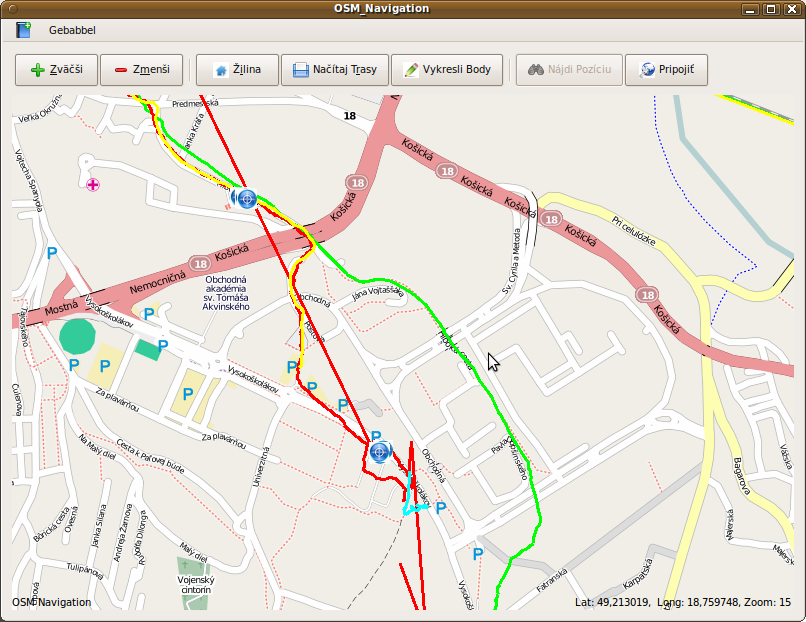
\includegraphics[width=14.5cm]{obr/mapa}
\caption{Trasa a významné body vykreslené na OSM mape}
\end{figure}



Pri zmenšení alebo zväčšení mapy musíme prekresliť na mape nové časti pretože pri priblížení alebo vzdialení sa nám mierkou zmenil obrázok na obrázok s iným detailom čo môžme spozorovať aj úplne iným snímkom.\\
Základné zmeny ktoré sa pri prekresľovaní dejú môžeme rozdeliť na dve časti: 
\begin{list}{•}
\item presúvanie sa po mape 
\item
\item zmena veľkosti mierky (`zoomovanie`)
\end{list}

\paragraph{Presúvanie sa po mape}
Program si pamätá jednu základnú súradnicu v jeho strede tzv. center. Od tejto súradnice sa odvíja celková poloha mapy ktorá je viditeľná.\\
Posun po mape je riešený dvoma spôsobmi:
\begin{list}{•}
\item posun klávesovými šípkami
\item
\item posun uchytením mapy myšou presun do žiadanej časti
\end{list}
Pri každej zmene mapy je potrebné v aplikačnej časti programu prepočítať nové hodnoty každej časti mapy. 


\paragraph{Zmena veľkosti mierky}
Ak chceme mapu zmenšiť, alebo zväčšiť môžeme tak urobiť viacerými spôsobmi:
\begin{list}{•}
\item dvojkliknutím na plochu mapy(ľavé tlačidlo priblíži mapu a pravé mapu vzdiali)
\item
\item rolovaním kolieskom myši 
\item kliknutím na tlačidlá priblíženia a vzdialenia
\end{list}
Pri týchto úkonoch sa vyvolávajú funkcie ktoré zmenia nastavenia priblíženia mapy (zoom-u) a následne sa vyvolá prekreslenie mapy.

\subsection{Pripojenie GPS zariadenia}
\paragraph{}
V tejto aplikácii existujú dve možnosti ako zariadenie pripojiť. Na výber nás v aplikácii vyzve podoknom (obr. 4.2). Prvá možnosť je pripojenie pomocou USB portu kde po pripojení vytvára OS port \textit{ttyUSB0}. Z tohto portu je možné čítať dáta vo forme NMEA protokolu. Druhou možnosťou je pripojiť zariadenie pomocou bezdrôtového pripojenia Bluetooth. V aplikácii je potrebné zadať MAC\footnote{\textbf{MAC} - Riadenie prístupu k médiu (Media Acces Control) = hardvérová adresa}. V prípade, že si v aplikácii zvolíme bezdrôtové pripojenie musíme zadať MAC adresu zariadenia (obr. 4.2). Po úspešnom pripojení už je možné čítať potrebné dáta.
\begin{figure}[ht]
\centering
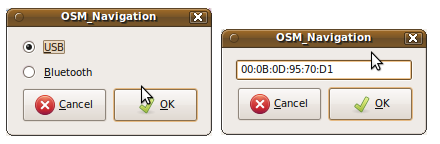
\includegraphics[width=12.5cm]{obr/volba_pris}
\caption{Výber spôsobu pripojenia}
\end{figure}


\subsection{Hľadanie aktuálnej pozície}
\paragraph{}
Hľadanie aktuálnej pozície má určitú postupnosť krokov. Ak je GPS zariadenie aktívne. Môže sa spustiť vyhľadávanie aktuálnej pozície. Príjem dát je riešený podprocesom ktorý spustí príkaz na čítanie dát z jedného z portu (USB – ttyUSB0, Bluetooth – rfcomm0).

Prístroj posiela dáta v protokole NMEA, dáta stačí rozdeliť a vhodne použiť na zistenie aktuálnej pozície. 

Po výzve používateľa sa výsledné dáta načítajú a pravidelne zobrazujú na mape. Vizuálnym výsledkom je mapa na ktorej je zobrazená naša aktuálna pozícia.
\begin{flushleft}
\textbf{Príkazy na čítanie dát:}
\begin{verbatim}
  cat /dev/rfcomm0  - v prípade pripojenia cez Bluetooth
  cat /dev/ttyUSB0  - v prípade zariadenia pripojeného cez USB
\end{verbatim}
\end{flushleft}

\section{Licencia aplikácie a požitých knižníc a programov}
\paragraph{}
V programe boli použité najme Knižnicou Qt , ktorá je pod licenciou GNU\footnote{\textbf{GNU} - } GPL~2\footnote{\textbf{GPL} - General public licence} pre nekomerčné využitie. 

Program Gebabbel má licenciu GNU GPL 2 a vlastník práv je Christoph Eckert. 
Program GPSbabel dovoľuje použitie pod licenciu GNU GPL 2, samotné časti programu môžu byť pod licenciu vlastníka samotnej časti.
   	% OSM Navigation
%\addcontentsline{toc}{}{}
\addcontentsline{toc}{chapter}{Záver}
\chapter*{Záver}
\paragraph{}
Úlohou v tejto práci bolo vytvorenie aplikácie ktorá bude schopná zobrazovať GPS dáta a komunikovať prístrojmi. Požiadavky na aplikáciu v jej prvej fáze môžme považovať za splnené. 
Ako ďalšie časy ktoré boli do aplikácie pridané sú multijazyčný preklad, ktorý je vhodný hlavne pri zdieľaní takejto aplikácie na internete. Aplikácia bude voľne dostupná, teda je možné ju využívať na študijné ale aj praktické účely pri zobrazovaní trás a aktuálnej pozície. 

Vo svojej prvej fáze je možné aplikáciu spúšťať na rôznych linuxových operačných systémoch v jej plnej funkčnosti. Aplikácia nie je náročná a je možné ju spúšťať aj pri menej výkonnom hardvéri. Samotné vykresľovanie trás je už v aktuálnej verzii plne funkčné aj pri iných platformách. 
\paragraph{}
V tejto práci sme si ozrejmili prácu s Qt knižnicou. Veľký prínos mala aj pre samotné geografické poznatky keďže sme sa často zaoberali výpočtami spoločnými s geografiou. 

Pri porovnávaní formátov sa nám ako najvhodnejší javí formát GPX a aj preto bola práve pre tento typ súboru podporovaná vizualizácia. Samotné programy ako gpsbabel majú podporu aj grafického rozhrania ktoré sa podarilo implementovať do samotnej aplikácie. Prevod dokáže hravo zvládnuť aj menej znalý používateľ tohto programu. 
\paragraph{}
Do budúcnosti je možné aplikáciu rozšíriť o ďalšie moduly, ktoré ju budú robiť komplexnejšou a robustnejšou.
   	% Záver
%\chapter*{Zoznam príloh}
%príloha č. 1 -- CD s popisovanými skriptami

%pri kopírovaní z www adries z tohto súboru odstrániť: \ znaky kde nepatria
\addcontentsline{toc}{chapter}{Literatúra}
\begin{thebibliography}{99}
%vzor
%[7] WIKIPEDIA: 23:09, 20. február 2010, Wikipedia: My SQL, 23:09, 20. február 2010.
%(http://sk.wikipedia.org/wiki/MySQL)
%1
\bibitem{GPSbabel}GPSbabel - časť skytraq datalogger. [2010] Dostupné na: \\
\verb|<|\emph{\url{http://www.gpsbabel.org/htmldoc-development/fmt\_skytraq.html}}\verb|>|
%\emph{} http://www.gpsbabel.org/htmldoc-development/The\_Formats.html
%2
\bibitem{GOL}Marián Jurík - GOL, diplomová práca . [2008] [Cit. 2010.2.22] Dostupné na:\\
\emph{univerzitná knižnica}
%3
\bibitem{GPX}GPX format   Dostupné na: \\
\verb|<|\emph{\url{http://www.topografix.com/gpx.asp}}\verb|>|
%4
\bibitem{GPX 2}GPX ďalšie informácie [2009] Dostupné na: \\
\verb|<|\emph{\url{http://wiki.geocaching.cz/index.php?title=GPX}}\verb|>|
%5
\bibitem{GoogleMaps}Google mapy. [2010] [Cit. 2010.4.16] Dostupné na: \\
\verb|<|\emph{\url{http://sk.wikipedia.org/wiki/Google\_Maps}}\verb|>|
%6
\bibitem{Kar Projekcia}Kartografická projekcia. [1996] Dostupné na: \\
\verb|<|\emph{\url{http://nic.sav.sk/logos/journals/geoinfo/0196/milan.html}}\verb|>|
%7
\bibitem{Qt class}Qt Classes. [2010] Dostupné na: \\
\verb|<|\emph{\url{http://doc.trolltech.com/3.3/classes.html}}\verb|>|
%8
\bibitem{Qtgraph}Qt Graphics dojo. [2008] Dostupné na:\\
\verb|<|\emph{\url{http://labs.trolltech.com/page/Graphics/About/Dojo}}\verb|>|
%9
\bibitem{OSM}Open Street mapy. [2010] [Cit. 2010.4.16] Dostupné na: \\
\verb|<|\emph{\url{http://sk.wikipedia.org/wiki/OpenStreetMap}}\verb|>|
%10
\bibitem{Slovník}Slovník pojmov týkajúcich sa GPS systému. [2010] [Cit. 2010.3.11] Dostupné na: 
\verb|<|\emph{\url{http://www.commander.sk/index.php?dok=0094}}\verb|>|
%11
\bibitem{GPS} Wikipédia: Global Positioning System. [2010] [Cit. 2010.4.7] Dostupné na: \verb|<|\emph{\url{http://sk.wikipedia.org/w/index.php?title=Global_Positioning_System&oldid=2923803}}\verb|>|
%12
\bibitem{WGS}Wikipédia:Svetový geodetický systém 1984 [2009][Cit. 2010.4.20]Dostupné na: \verb|<|\emph{\url{http://sk.wikipedia.org/wiki/Svetový\_geodetický\_systém\_1984}}\verb|>|
%13
\bibitem{Bluetooth}Navilock GPS Bluetooth Receiver BT-308. [2010] Dostupné na: 
\verb|<|\emph{\url{http://www.gpstechnologies.com.au/bt308.htm}}\verb|>|
%14
\bibitem{NMEA}Protokol NMEA, popis. [2010] Dostupné na: \\
\verb|<|\emph{\url{http://www.kh-gps.de/nmea-faq.htm}}\verb|>|

%15
\bibitem{GPS}GPS MULTITRACKER manual( MT5013 )[online]. [s.a.] [Cit. 2010.3.11] Dostupné na: \\
\verb|<|\emph{\url{http://www.media-tech.eu/upload/manuals/MT5013_EN_user_manual.pdf}}\verb|>|


%\verb|<|\emph{\url{http://www.google.sk/url?sa=t&source=web&ct=res&cd=1&ved=0CBcQFjAA&url=http\%3A\%2F\%2Fwww.media-tech.eu\%2Fupload\%2Fmanuals%2FMT5013_EN_user_manual.pdf&ei=OGDlS5zBAo6mOJv00OUN&usg=AFQjCNF7g6LukSgT6to8LIGI6b-_fzqfIg&sig2=BwRBPIlCSX8FeINcMHOJtg}}\verb|>|

\end{thebibliography}  % literatura
\addcontentsline{toc}{chapter}{Zoznam použitých skratiek}
\newpage
\chapter*{Zoznam použitých skratiek}


\thispagestyle{empty}

\textbf{GPS} - globálny pozičný systém\\
\textbf{OSM} - Open street map\\
\textbf{NMEA} - national marine electronic association\\
\textbf{GPX} - GPS eXchange format = formát na výmenu dát\\
\textbf{OS} - Operačný systém\\
\textbf{WGS-84} - World Geodetic System 1984\\
\textbf{NAVSTAR GPS} - NAVigation Signal for Timing And Ranging\\
\textbf{GLONASS} - Globálny satelitný navigačný systém\\
\textbf{XML} - eXtensible Markup Language(rozšíriteľný značkovací jazyk)\\
\textbf{HTML} - HyperText Markup Language(Hypertextový značkový jazyk )\\
\textbf{USB} - Univerzálna sériová zbernica (Universal serial bus)\\
\textbf{MAC} - Riadenie prístupu k médiu (Media Acces Control) = hardvérová adresa\\
\textbf{GNU} - „GNU Nie je Unix“ (angl. „GNU's Not Unix“)\\
\textbf{GPL} - General public licence\\

   	% zoznam použitých skratiek
\listoffigures    	% zoznam obrazkov
\chapter*{Prílohy}
\addcontentsline{toc}{chapter}{Prílohy}

\textbf{DVD obsahujúce:}
\begin{enumerate}
\item Elektronickú verziu bakalárskej práce
\item Inštalačný balík programu OSM\_Navigation
\item Používateľská a programátorská príručka s návodmi na inštaláciu
\end{enumerate}



    
    
	% zoznam priloh k bakalárke
\chapter*{}
\thispagestyle{empty}
%\vfill
\vspace{4cm}
Súhlasím, aby sa bakalárska práca s názvom Softvér pre komunikáciu s GPS modulom a zobrazovanie GPS dát požičiavala v knižnici na študijné účely.


\vspace{10cm}
\noindent
V Žiline dňa \makebox[8em]{\dotfill} 
\begin{flushright}
\hfill Podpis\makebox[8em]{\dotfill}\\
\hfill Dušan Ščensný 
\end{flushright}

	% suhlas o zverejneni

\end{document}
